\subsection{Collaborative Evidence Schematization}

Participants believed the visualization tools provided by CAnalytics facilitated the schematization and synthesis process. When they created a data object, the data was automatically laid out in multiple views. This changes their workflow from linear (first extract data and then visualize data) to parallel (create and view data objects). When a team is collecting evidence from the document, they are also organizing the document with sorted evidence. 

\begin{quote}
	\textit{`CAnalytics is helpful to our work because of its ability to edit the physical document with such organization. This with the combination of immediately adding all of the entities into a connected web that doesn't have to be manually created saves a lot of time'.} (P10)
\end{quote}

Another benefit students mentioned was that they no longer needed to create separate data structures redundantly for different analytic tools. To visualize different data types (e.g. spatial data, event data, linked data), analysts have multiple tools in their toolkit, yet different tools usually require different data formats. 

\hl{quote supporting the argument that team do not need to create separate models}

Besides, traditional visualization tools are usually designed for single user only. Thus teams had to divide work by tools; for example, one member creates an ACH matrix, and another member creates a node-link graph. The tool limit leads to loose coupled collaborative work; individuals work on their own and put together work in the end. 

\begin{quote}
	\textit{`we split the work by category: one would do the timeline, one would write up assumptions, and one would work on the IEW chart. We did this since all of us could not edit a single document at the same time.'}
\end{quote}

Using multiple tools also results in multiple scattered documents, making it difficult for teams to manage and organize.  

\begin{quote}
	\textit{`When we didn't have CAnalytics, we had a lot of different word documents that we had to share with each other in Google Doc. With CAnalytics, we were able to keep all the information, network, timeline, and BLUF analysis in one spot that we were all able to view at the same time as a group'.} (P58)
\end{quote}
\begin{quote}
	\textit{`CAnalytics made it easier to see everything mapped out in one place as opposed to doing it the old fashion way. It was way more convenient and efficient to have everything in one application'.} (P71)
\end{quote}


% The ease of sharing and putting work together also helps information analysis. Students found it helpful ``because I could see how all of our different ideas merged together to create our final product.'' Another student shared his experience about how the tool helped develop their theory. 


The positive feedback from the questionnaire is confirmed with system logs. We find that the usage of visualization tools is significantly correlated with team performance (r = .49, p < .05). Note we exclude Team 78, 79, 93, 109, and 111 as outliers as they did not use much of the tool. 

\begin{figure}
	\centering
	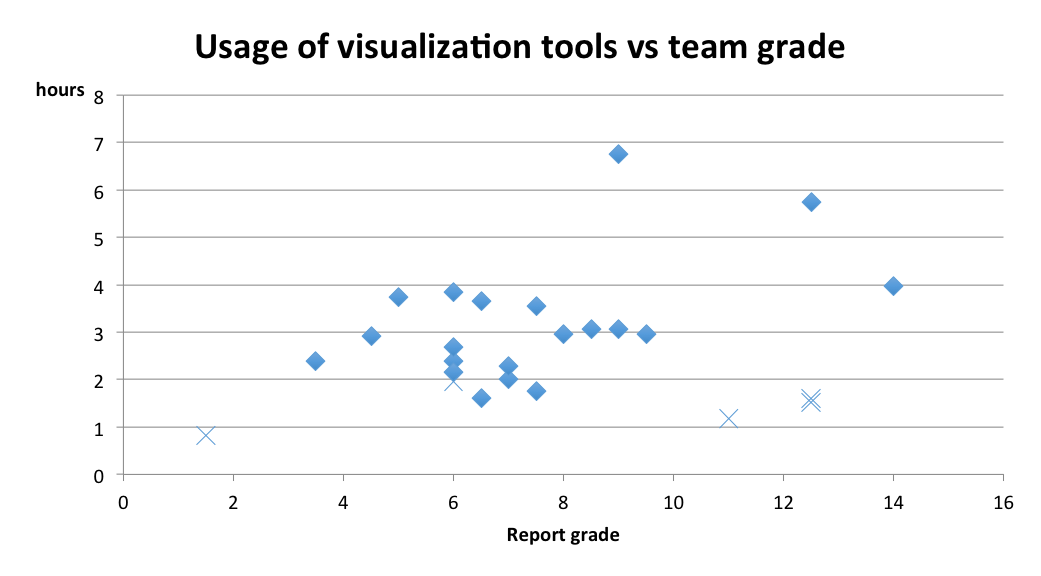
\includegraphics[height=1.5in]{img/vis_correlate_perf}
	\caption{Chart showing that team performance is highly correlated with usage of visualization tools (r = .49, p < .05). Crossings are outlier teams that do not use much of visualization tools}
\end{figure}

\hl{visualization usage??}
We then look into more specifically how teams used the visualization tools. Teams spent most time on the node-link graph. 

\begin{figure}
	\centering
	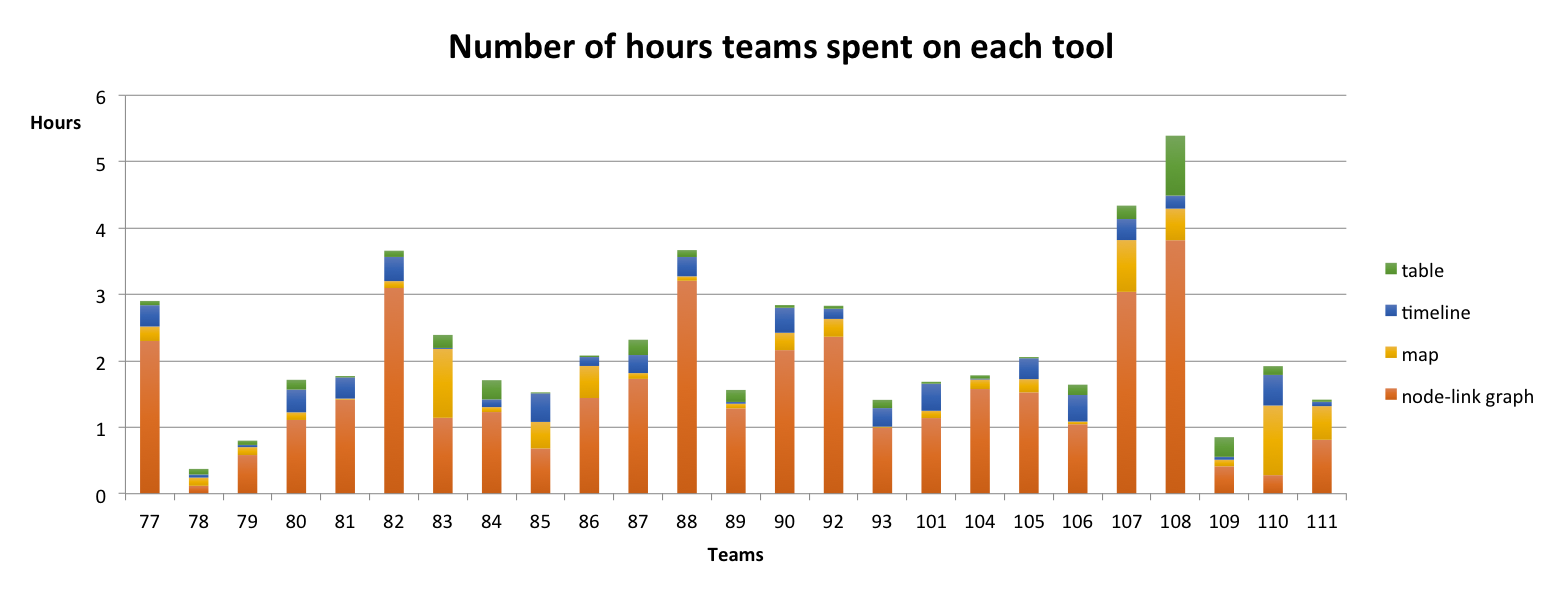
\includegraphics[height=1.5in]{img/vis_usage}
	\caption{Chart showing the usage of the visualization tools}
\end{figure}

When we look into the visualization products team created, we find several problems. For example, when information volume increases, it becomes challenging to distinguish useful information from background noise. As shown in the top graph in Figure~\ref{fig:network_example}, the node-link graph contains so many nodes that pattern discovery becomes very difficult.



%% reliability of information 
Another issue is difficulty to distinguish reliability of information. For example, while all displayed as valid connections in the node-link graph, some connections were literally specified in the original document, whereas others might be inferred. Analysts must be cautious about the different reliability of these connections when taking them for analysis. To avoid the issue, some groups only added most reliable facts to the shared view. While this approach kept the graph clean and free of noise, the team lost the chance to get inspired by and build upon each other's thought, which is of critical value in collaborative information analysis. Worse, the fear that adding a piece of less reliable information would mislead group thinking would discourage teammates to contribute. Mechanism to share and distinguish information of mixed reliability is needed.


Participants also complaint that not being able to share the schematization result makes their collaboration difficult. The current design allows individuals to arrange their own layout of evidence without interfering other member's sensemaking. However, while acknowledging the advantage of parallel sensemaking, participants requested to be able to share their visual product so that they can discuss based on the same ground.

\begin{quote}
	This was very hard to coordinate with my group members because we could be looking at the same information but arranged in completely different ways. (User 31)
\end{quote}

